\chapter{Numerical Needle Probe Approach}
\label{sec:numerical-np}
\bigskip

\section{Introduction} 
\label{sec:numerical-np:introduction}

Numerical experiments were used to simulate needle probes in anisotropic mediums with
three-dimensional finite element heat transfer models in COMSOL 3.5a. These
consisted of a large-scale parametric study using varying combinations of \(k_{xy}\), \(k_z\) and angle orientation \(\theta\).

\section{Geometry and Domain Properties}
\label{sec:numerical-np:domain}

\begin{figure}[h]
\centering
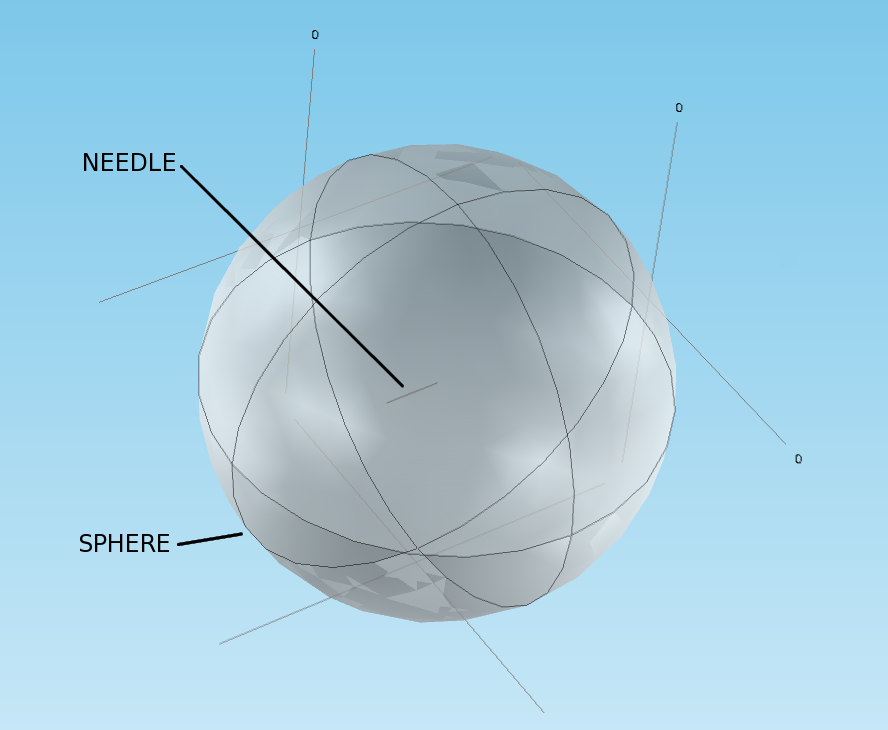
\includegraphics[width=0.8\textwidth]{fig/domain_2.png}
\caption{A COMSOL screenshot showing the geometry of the finite element model, which consists of a metal needle in a sphere of a snow-like material.}
\label{fig:domain}
\end{figure}


\begin{table}[h]
\centering
\caption{Constants used in numerical models.}
\begin{tabular}{r | l}
radius of needle & \(0.25\) mm\\
length of needle & \(10\) cm\\
radius of snow & \(40\) cm\\
\hline
density of needle & \(8000\) kg/\(\textrm{m}^3\)\\
\(C_P\) of needle & \(460\) \(\flatfrac{\textrm{J}}{\textrm{kg}\cdot\textrm{K}}\) \\
\(q\) of needle & \(0.5\) W/m\\
\(k\) of needle & \(160\) W/m\(\cdot\)K\\
\hline
density of snow & \(200\) kg/\(\textrm{m}^3\)\\
\(C_P\) of snow & \(2050\)  \(\flatfrac{\textrm{J}}{\textrm{kg}\cdot\textrm{K}}\)
\end{tabular}
\label{tab:constants}
\end{table}

The needle is simulated as a long, thin steel cylinder embedded in the center
of a sphere of a snow-like material (called snow in this model), as in Figure \ref{fig:domain}. While most of the dimensions
and material properties are held constant (see Table \ref{tab:constants}), the
anisotropic conductivity of the snow is parameterized in the form
of a  \(3\times3\) symmetric matrix with all positive eigenvalues.  In practice, this is
done by specifying a diagonal matrix \(\Lambda\) with positive eigenvalues
\(k_{xy}\) and \(k_z\) and a rotation matrix \(R\) around the \(x\) axis, and
then defining \(K = R^T\Lambda R\) as in Equation \ref{eq:rotdiagrot} :

\begin{equation}
\label{eq:rotdiagrot}
K = \begin{bmatrix}
\cos(\theta) & 0 & \sin(\theta)\\
0 & 1 & 0\\
-\sin(\theta) & 0 &\cos(\theta)
\end{bmatrix}
\begin{bmatrix}
k_{xy} & 0 & 0\\
0 & k_{xy} & 0\\
0 & 0 & k_z
\end{bmatrix}
\begin{bmatrix}
\cos(\theta) & 0 & -\sin(\theta)\\
0 & 1 & 0\\
\sin(\theta) & 0 &\cos(\theta)
\end{bmatrix}
\end{equation}

The boundary conditions on the surface of the sphere enforce zero heat flux,
and the radius of the sphere is chosen such that the sphere approximates an
infinite medium.

Point temperatures recorded are the center of the needle, which corresponds to
the location of the thermocouple used in real-world experiments, and six points
on the surface of the snow, to ensure that the sphere is sufficiently large by
checking for a near-zero increase in temperatures on these points. In these
models, the increase in temperature is on the order of \(10^{-14}\) degrees
Kelvin.

\section{MATLAB in Geometry-Based Parametric Studies Using COMSOL 3.5a}
\label{sec:numerical-np:matlab}

Unfortunately, COMSOL 3.5a does not have the facilities necessary to implement a
geometry-changing multi-parameter parametric study as required from the GUI alone. However,
COMSOL 3.5a does have facilities for scripting with MATLAB.

MATLAB code written to implement the parametric study was largely auto-generated
by COMSOL, by building a base model in COMSOL 3.5a and exporting to an m-file.
This code is split into two parts: The meshing code, and the solving code.
These pieces of code are wrapped in functions, called ``mesher'' and ``solver''
respectively, and used by a main procedure called ``worker.m.''

\begin{figure}[h]
\centering
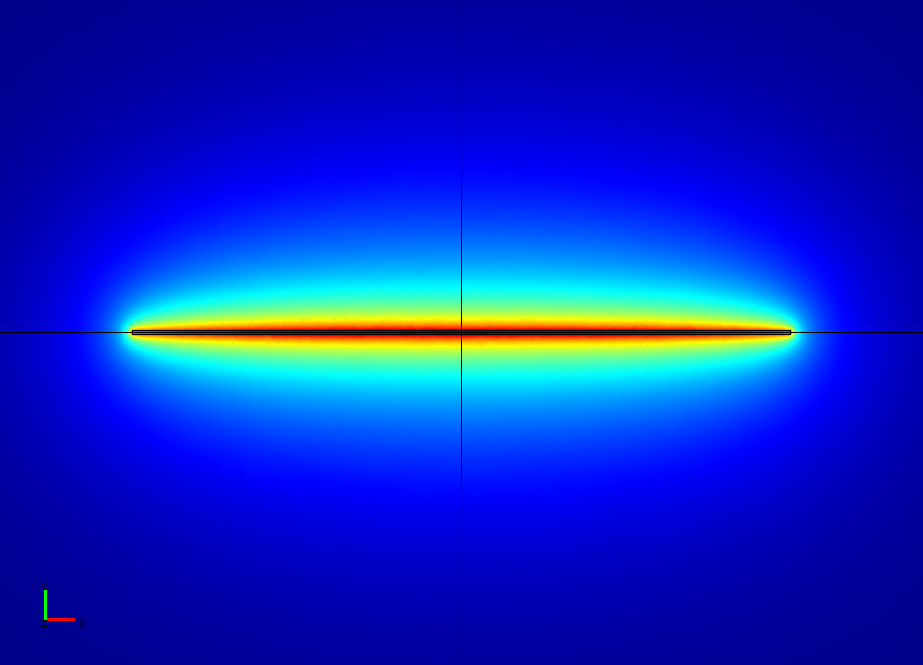
\includegraphics[width=0.6\textwidth]{fig/35892_elem_1097s.png}
\caption{A side-view of COMSOL's results, focusing on the needle. Colors indicate temperature.}
\label{fig:comsol}
\end{figure}

\section{Automatic Calculation of Conductivity from Simulated Time/Temperature Data}

Results from COMSOL are automatically fitted against the linear model with
respect to \(\ln(t)\) by ``dropping'' early \((t,T)\) datapoints until the
correlation coefficient of the remaining points was sufficiently high, as in Figure \ref{fig:curvefit}. Then, a
linear curvefit is applied to these remaining points. Finally, the slope of this fit is
used to calculate \(k_{\textrm{eff}}\).

\begin{figure}[h]
\centering
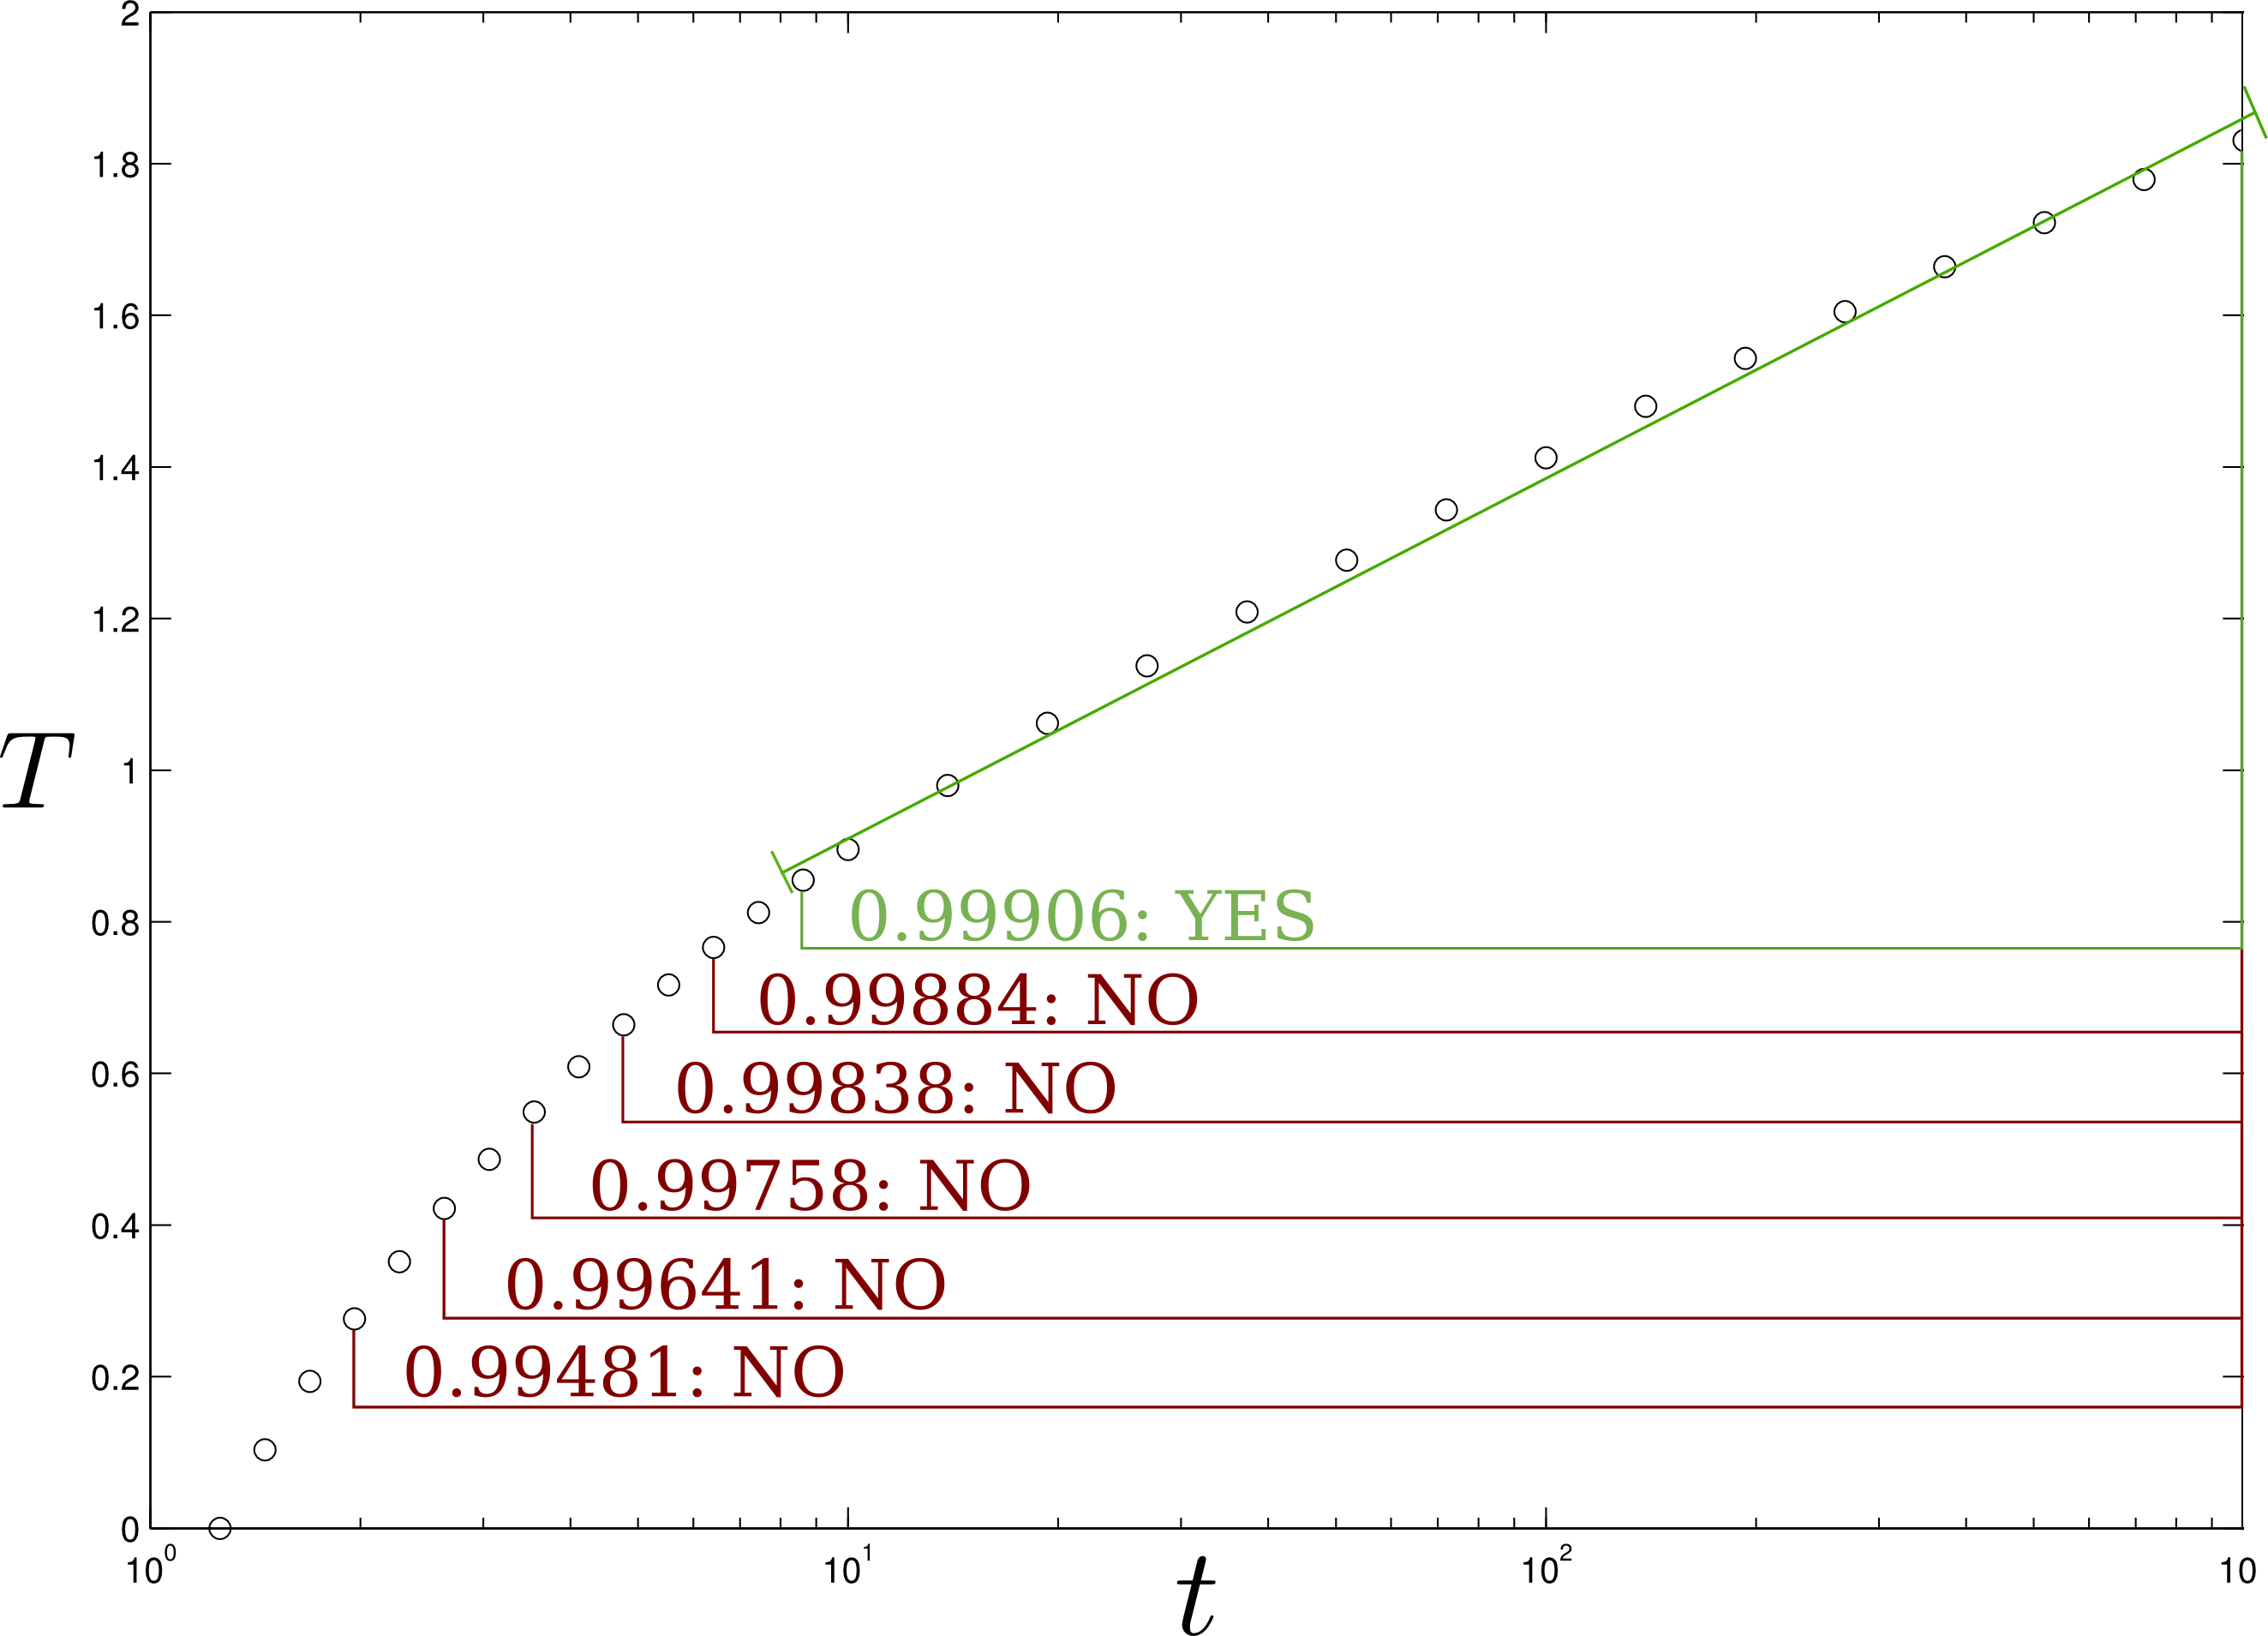
\includegraphics[width=0.6\textwidth]{fig/curvefit.png}
\caption{An illustration of the method used to find the "long-time" slope of the numerical simulations, which used a correlation coefficient to estimate the "straightness" of a section.}
\label{fig:curvefit}
\end{figure}

The results from these analyses are organized into a nested
cell array which mirrors the format of the two MATLAB matrices k\_xy and k\_z.
The data in each slot of the
nested array is itself a cell array containing the simulation results, organized as shown
in Figure \ref{fig:cellarray}. Typically, the only data saved from the simulation was the \((t,T)\) data from the center of the modeled needle, the average of the temperatures on the surface of the sphere, and the simulated \(k_{\textrm{eff}}\). In some runs, the raw structure representing the problem to COMSOL was exported back to the native .mph format for
further study, such as viewing the temperature distribution over the entire
domain as in Figure \ref{fig:comsol}. 


\begin{figure}

\centering
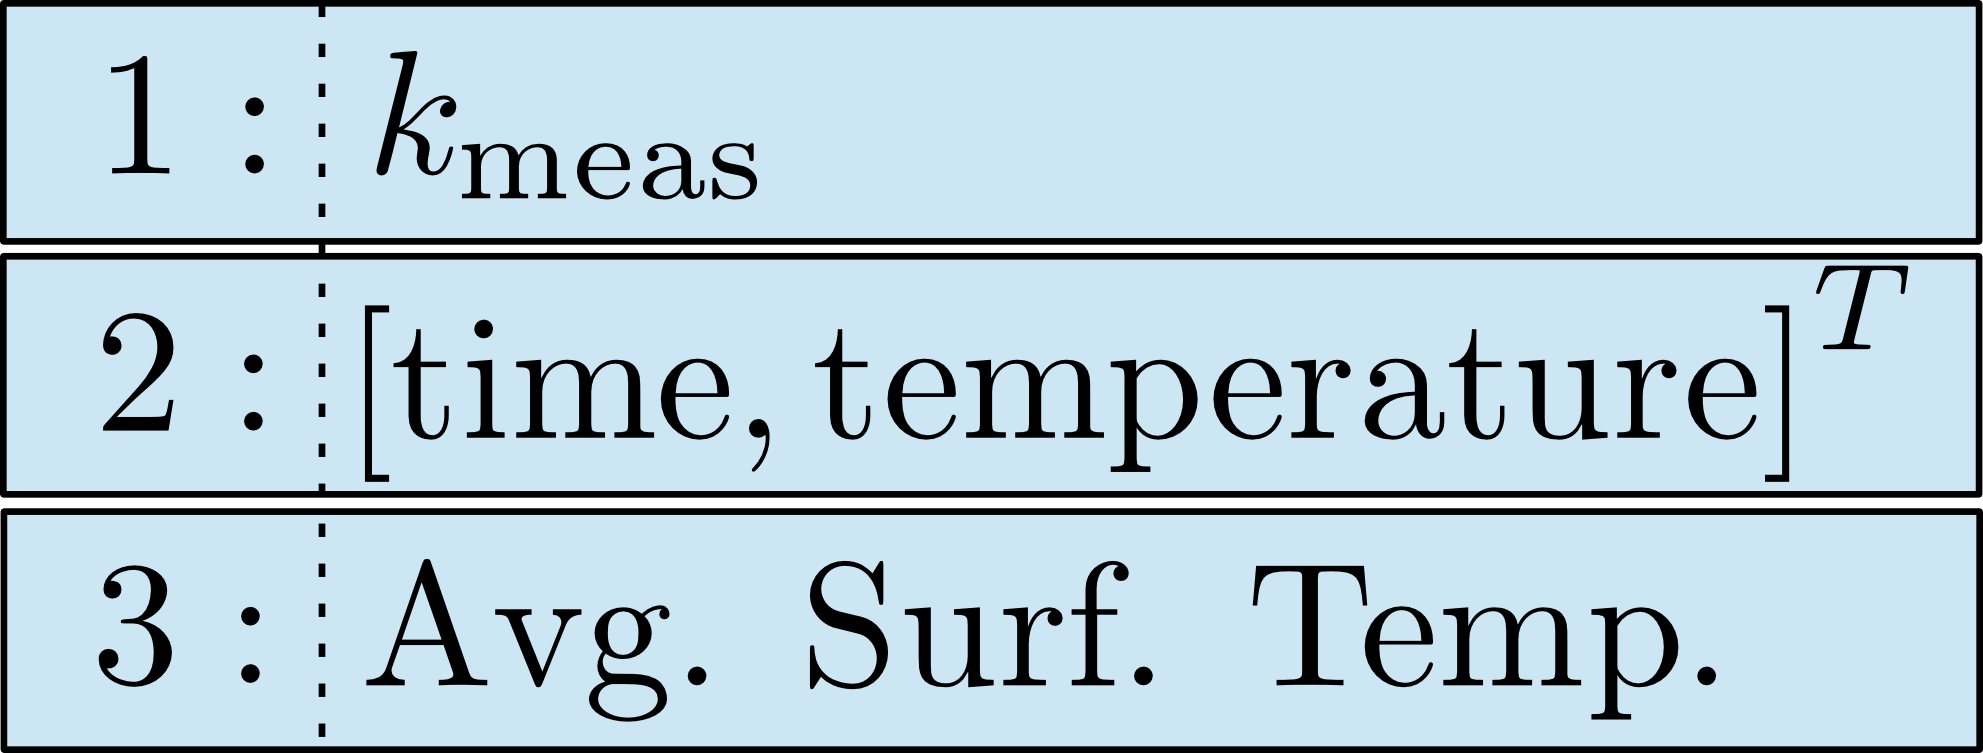
\includegraphics[width=0.25\textwidth]{fig/cellarray.png}
\caption{Contents of a cell array, representing the results of a particular simulation.}
\label{fig:cellarray}
\end{figure}

A number of analyses, some of more use than others, can be applied to the
data. For example, one procedure applied asserted that all averaged sphere
surface temperatures had increased by less than a thousandth of a degree.

\section{Convergence Study}

A small, informal convergence study was executed in order to get a general idea
of how appropriate the model's chosen grid size is. A convergence study, in this
context, consists of running the same model with different grid sizes and
studying how the results change as a function of grid size.  The goal is to show
that the problem converges on a particular solution when grid size is
sufficiently refined. While this can't prove that the solution being converged
to is the \emph{correct} solution, it can show that, given that the convergent
solution is correct, that the model uses a sufficiently refined grid to get
sufficiently accurate results.

For this convergence study, a particular solution was chosen from the finite
element parametric study and the mesh was refined to different levels. An
analysis of these results should then give an idea of the convergence properties
of the problem.

One issue that occurs with such convergence studies is that refining the grid
exponentially increases the difficulty of solving the resulting finite element
model. In this instance, the grid could only be refined once without reaching
a point where solving the problem became impractical. This gives only two data
points for which to base any conclusions, but even this may be useful.

\begin{table}[h]
\centering
\caption{It quickly becomes impractical to increase the mesh size of a model, as
increases in runtime are non-linear and are limited by both CPU and computer memory.}
\begin{tabular}{r | l}
Number of Elements & Time to Complete\\
\(35892\) elements & \(\approx 10\) minutes\\
\(159641\) elements & \(\approx 2\) hours\\
\(528945\) elements & ??? (\(>3\) weeks)\\
\end{tabular}

\label{tab:conv_runtime}
\end{table}

\section{Conclusions}

COMSOL 3.5a is used to run three-dimensional simulations of thermal conduction
in the needle probe problem, in concert with MATLAB for automation and
post-processing. The method generated
useful information on predicted thermal conductivity measurements from a heating
curve approach given an anisotropy and a needle orientation with respect to this
needle orientation.
